\documentclass{standalone}
\usepackage{tikz}
\usetikzlibrary{patterns, positioning}
\usepackage[sfdefault]{ClearSans} %% option 'sfdefault' activates Clear Sans as the default text font
\usepackage[T1]{fontenc}

\begin{document}
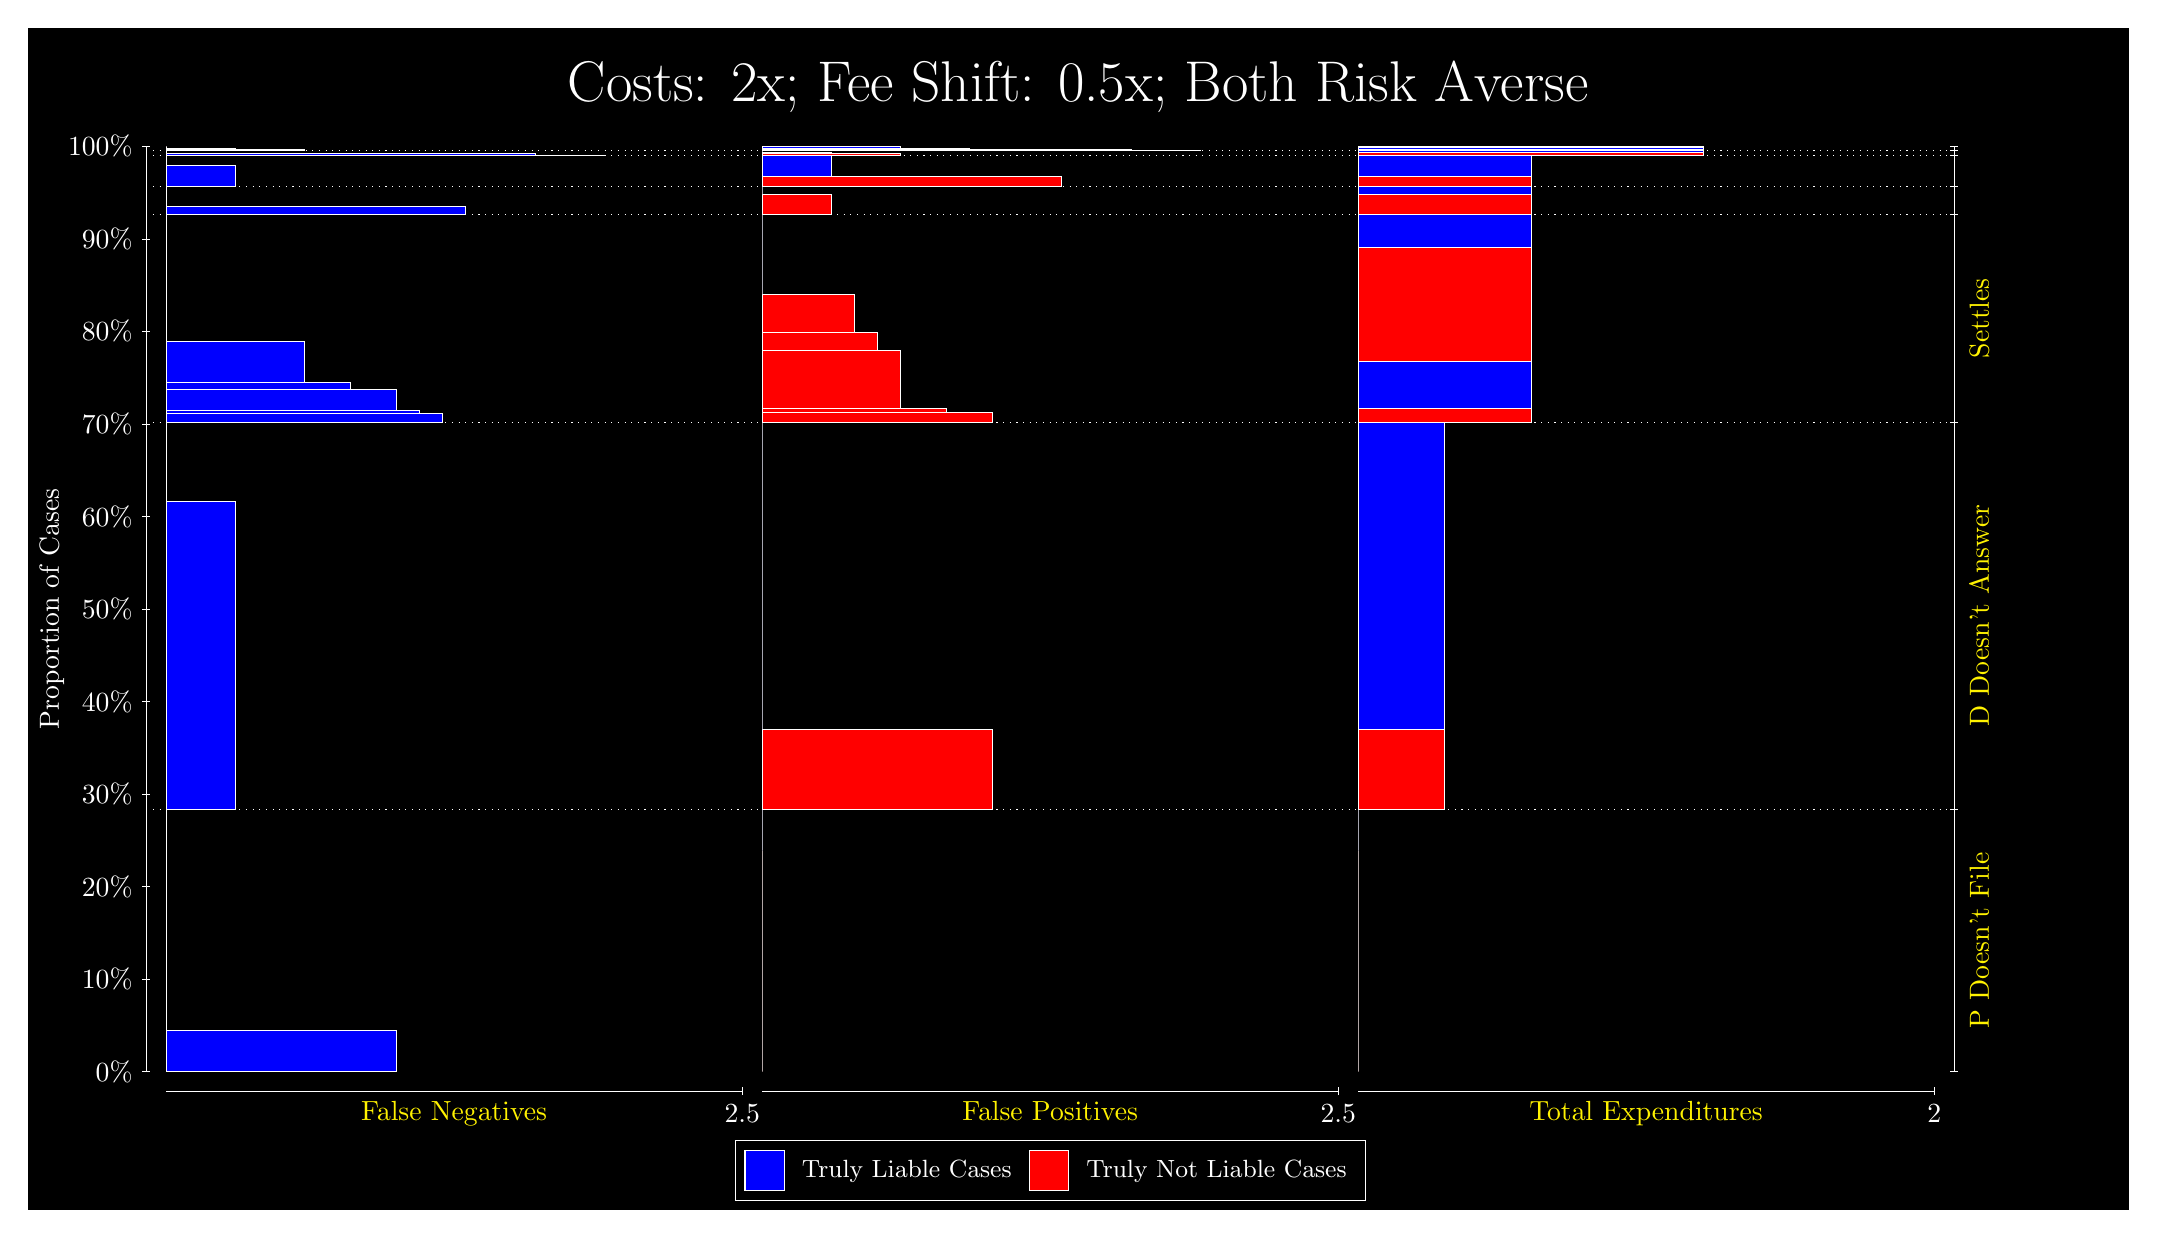
\begin{tikzpicture}
\draw[fill=black] (0,0) rectangle (26.667,15);
\draw[text=white] (0,13.5) rectangle (26.667,15) node[midway] {\huge Costs: 2x; Fee Shift: 0.5x; Both Risk Averse};
\draw[white, very thin] (1.5,1.75) -- (1.5,13.5);
\node[rotate=90, text=white, anchor=center] at (0.3, 7.625) {Proportion of Cases};
\draw[white, very thin] (1.45,1.75) -- (1.55,1.75);
\node[text=white, anchor=east] at (1.45, 1.75) {0\%};
\draw[white, very thin] (1.45,2.925) -- (1.55,2.925);
\node[text=white, anchor=east] at (1.45, 2.925) {10\%};
\draw[white, very thin] (1.45,4.1) -- (1.55,4.1);
\node[text=white, anchor=east] at (1.45, 4.1) {20\%};
\draw[white, very thin] (1.45,5.275) -- (1.55,5.275);
\node[text=white, anchor=east] at (1.45, 5.275) {30\%};
\draw[white, very thin] (1.45,6.45) -- (1.55,6.45);
\node[text=white, anchor=east] at (1.45, 6.45) {40\%};
\draw[white, very thin] (1.45,7.625) -- (1.55,7.625);
\node[text=white, anchor=east] at (1.45, 7.625) {50\%};
\draw[white, very thin] (1.45,8.8) -- (1.55,8.8);
\node[text=white, anchor=east] at (1.45, 8.8) {60\%};
\draw[white, very thin] (1.45,9.975) -- (1.55,9.975);
\node[text=white, anchor=east] at (1.45, 9.975) {70\%};
\draw[white, very thin] (1.45,11.15) -- (1.55,11.15);
\node[text=white, anchor=east] at (1.45, 11.15) {80\%};
\draw[white, very thin] (1.45,12.325) -- (1.55,12.325);
\node[text=white, anchor=east] at (1.45, 12.325) {90\%};
\draw[white, very thin] (1.45,13.5) -- (1.55,13.5);
\node[text=white, anchor=east] at (1.45, 13.5) {100\%};

\draw[white, very thin] (24.457,1.75) -- (24.457,13.5);
\draw[white, very thin] (24.407,1.75) -- (24.507,1.75);
\node[anchor=west] at (24.407, 1.75) {};
\draw[white, very thin] (24.407,5.0798) -- (24.507,5.0798);
\node[anchor=west] at (24.407, 5.0798) {};
\draw[white, very thin] (24.407,9.997) -- (24.507,9.997);
\node[anchor=west] at (24.407, 9.997) {};
\draw[white, very thin] (24.407,12.637) -- (24.507,12.637);
\node[anchor=west] at (24.407, 12.637) {};
\draw[white, very thin] (24.407,12.991) -- (24.507,12.991);
\node[anchor=west] at (24.407, 12.991) {};
\draw[white, very thin] (24.407,13.388) -- (24.507,13.388);
\node[anchor=west] at (24.407, 13.388) {};
\draw[white, very thin] (24.407,13.447) -- (24.507,13.447);
\node[anchor=west] at (24.407, 13.447) {};
\draw[white, very thin] (24.407,13.5) -- (24.507,13.5);
\node[anchor=west] at (24.407, 13.5) {};

\draw[white, very thin, fill=blue] (1.75,1.75) rectangle (4.6775,2.2744);
\draw[white, very thin, fill=red] (1.75,2.2744) rectangle (1.75,5.0798);
\draw[white, very thin, fill=blue] (1.75,5.0798) rectangle (2.6283,8.9859);
\draw[white, very thin, fill=red] (1.75,8.9859) rectangle (1.75,9.997);
\draw[white, very thin, fill=blue] (1.75,9.997) rectangle (5.2631,10.104);
\draw[white, very thin, fill=blue] (1.75,10.104) rectangle (4.9703,10.152);
\draw[white, very thin, fill=blue] (1.75,10.152) rectangle (4.6775,10.42);
\draw[white, very thin, fill=blue] (1.75,10.42) rectangle (4.092,10.505);
\draw[white, very thin, fill=blue] (1.75,10.505) rectangle (3.5065,11.019);
\draw[white, very thin, fill=red] (1.75,11.019) rectangle (1.75,12.637);
\draw[white, very thin, fill=blue] (1.75,12.637) rectangle (5.5558,12.743);
\draw[white, very thin, fill=red] (1.75,12.743) rectangle (1.75,12.991);
\draw[white, very thin, fill=blue] (1.75,12.991) rectangle (2.6283,13.255);
\draw[white, very thin, fill=red] (1.75,13.255) rectangle (1.75,13.388);
\draw[white, very thin, fill=blue] (1.75,13.388) rectangle (7.3123,13.392);
\draw[white, very thin, fill=blue] (1.75,13.392) rectangle (6.4341,13.407);
\draw[white, very thin, fill=red] (1.75,13.407) rectangle (1.75,13.447);
\draw[white, very thin, fill=blue] (1.75,13.447) rectangle (3.5065,13.468);
\draw[white, very thin, fill=blue] (1.75,13.468) rectangle (2.6283,13.481);
\draw[white, very thin, fill=red] (1.75,13.481) rectangle (1.75,13.5);
\draw[white, very thin, fill=red] (9.3189,1.75) rectangle (9.3189,4.5555);
\draw[white, very thin, fill=blue] (9.3189,4.5555) rectangle (9.3189,5.0798);
\draw[white, very thin, fill=red] (9.3189,5.0798) rectangle (12.246,6.0909);
\draw[white, very thin, fill=blue] (9.3189,6.0909) rectangle (9.3189,9.997);
\draw[white, very thin, fill=red] (9.3189,9.997) rectangle (12.246,10.123);
\draw[white, very thin, fill=red] (9.3189,10.123) rectangle (11.661,10.172);
\draw[white, very thin, fill=red] (9.3189,10.172) rectangle (11.075,10.916);
\draw[white, very thin, fill=red] (9.3189,10.916) rectangle (10.783,11.144);
\draw[white, very thin, fill=red] (9.3189,11.144) rectangle (10.49,11.616);
\draw[white, very thin, fill=blue] (9.3189,11.616) rectangle (9.3189,12.637);
\draw[white, very thin, fill=red] (9.3189,12.637) rectangle (10.197,12.885);
\draw[white, very thin, fill=blue] (9.3189,12.885) rectangle (9.3189,12.991);
\draw[white, very thin, fill=red] (9.3189,12.991) rectangle (13.125,13.124);
\draw[white, very thin, fill=blue] (9.3189,13.124) rectangle (10.197,13.388);
\draw[white, very thin, fill=red] (9.3189,13.388) rectangle (11.075,13.411);
\draw[white, very thin, fill=red] (9.3189,13.411) rectangle (10.197,13.428);
\draw[white, very thin, fill=blue] (9.3189,13.428) rectangle (9.3189,13.447);
\draw[white, very thin, fill=red] (9.3189,13.447) rectangle (14.881,13.451);
\draw[white, very thin, fill=red] (9.3189,13.451) rectangle (14.003,13.466);
\draw[white, very thin, fill=blue] (9.3189,13.466) rectangle (11.954,13.479);
\draw[white, very thin, fill=blue] (9.3189,13.479) rectangle (11.075,13.5);
\draw[white, very thin, fill=red] (16.888,1.75) rectangle (16.888,4.5555);
\draw[white, very thin, fill=blue] (16.888,4.5555) rectangle (16.888,5.0798);
\draw[white, very thin, fill=red] (16.888,5.0798) rectangle (17.986,6.0909);
\draw[white, very thin, fill=blue] (16.888,6.0909) rectangle (17.986,9.997);
\draw[white, very thin, fill=red] (16.888,9.997) rectangle (19.083,10.172);
\draw[white, very thin, fill=blue] (16.888,10.172) rectangle (19.083,10.77);
\draw[white, very thin, fill=red] (16.888,10.77) rectangle (19.083,12.214);
\draw[white, very thin, fill=blue] (16.888,12.214) rectangle (19.083,12.637);
\draw[white, very thin, fill=red] (16.888,12.637) rectangle (19.083,12.885);
\draw[white, very thin, fill=blue] (16.888,12.885) rectangle (19.083,12.991);
\draw[white, very thin, fill=red] (16.888,12.991) rectangle (19.083,13.124);
\draw[white, very thin, fill=blue] (16.888,13.124) rectangle (19.083,13.388);
\draw[white, very thin, fill=red] (16.888,13.388) rectangle (21.279,13.428);
\draw[white, very thin, fill=blue] (16.888,13.428) rectangle (21.279,13.447);
\draw[white, very thin, fill=red] (16.888,13.447) rectangle (21.279,13.462);
\draw[white, very thin, fill=blue] (16.888,13.462) rectangle (21.279,13.482);
\draw[white, very thin, fill=red] (16.888,13.482) rectangle (21.279,13.487);
\draw[white, very thin, fill=blue] (16.888,13.487) rectangle (21.279,13.5);
\draw[white, dotted] (1.5,5.0798) -- (24.457,5.0798);
\draw[white, dotted] (1.5,9.997) -- (24.457,9.997);
\draw[white, dotted] (1.5,12.637) -- (24.457,12.637);
\draw[white, dotted] (1.5,12.991) -- (24.457,12.991);
\draw[white, dotted] (1.5,13.388) -- (24.457,13.388);
\draw[white, dotted] (1.5,13.447) -- (24.457,13.447);
\draw[white, very thin] (1.75,1.5) -- (9.0689,1.5);
\node[text=yellow, anchor=north] at (5.4094, 1.5) {False Negatives};
\draw[white, very thin] (9.0689,1.45) -- (9.0689,1.55);
\node[text=white, anchor=north] at (9.0689, 1.45) {2.5};

\draw[white, very thin] (9.3189,1.5) -- (16.638,1.5);
\node[text=yellow, anchor=north] at (12.978, 1.5) {False Positives};
\draw[white, very thin] (16.638,1.45) -- (16.638,1.55);
\node[text=white, anchor=north] at (16.638, 1.45) {2.5};

\draw[white, very thin] (16.888,1.5) -- (24.207,1.5);
\node[text=yellow, anchor=north] at (20.547, 1.5) {Total Expenditures};
\draw[white, very thin] (24.207,1.45) -- (24.207,1.55);
\node[text=white, anchor=north] at (24.207, 1.45) {2};

\node[text=yellow, centered, rotate=90] at (24.777, 3.4149) {P Doesn't File};
\node[text=yellow, centered, rotate=90] at (24.777, 7.5384) {D Doesn't Answer};
\node[text=yellow, centered, rotate=90] at (24.777, 11.317) {Settles};





\draw (12.978300999999998,1.5) node[draw=none] (baseCoordinate) {};
\begin{scope}[align=center]
        \matrix[scale=0.5, draw=white, below=0.5cm of baseCoordinate, nodes={draw}, column sep=0.1cm]{
            \node[rectangle, draw, minimum width=0.5cm, minimum height=0.5cm, fill=blue] {}; &
            \node[draw=none, font=\small, text=white] (B) {Truly Liable Cases}; &
            \node[rectangle, draw, minimum width=0.5cm, minimum height=0.5cm, fill=red] {}; &
            \node[draw=none, font=\small, text=white] (B) {Truly Not Liable Cases}; \\
            };
\end{scope}

\end{tikzpicture}
\end{document}